\chapter{Analysis of Resource-centric Organizational Modeling}
\label{chap:analysis}
This chapter positions the thesis work in the field of process modeling with respect to the other existing approach. The first section provides detailed requirement analysis about the research objectives described in Chapter \ref{chap:introduction}. The final section provides a detailed literature review about the existing approaches. A detailed evaluation of the existing approaches with the proposed requirements is also provided in this section.

%%%%%%%%%%%%%%%%%%%%%%%%%%%%%%%%%%%%%%%%%%%%%%%%%%%%%%%%%%%%%%%%%%%%%%%%%
\section{Requirements Analysis}
\label{sec:requirementssupoorting}
%%%%%%%%%%%%%%%%%%%%%%%%%%%%%%%%%%%%%%%%%%%%%%%%%%%%%%%%%%%%%%%%%%%%%%%%%
This section provides a detailed requirement analysis of research objectives mentioned in Chapter \ref{chap:introduction}. The below mentioned requirements are also satisfied by the functioning system developed through proposed approach in the following Chapter \ref{chap:approach}. Also the exact business process life cycle phase from the Figure \ref{fig:businessprocesslifecycle} when each of the requirements get satisfied are provided in Table \ref{tab:subrequirements}.

\begin{figure}
	\centering
	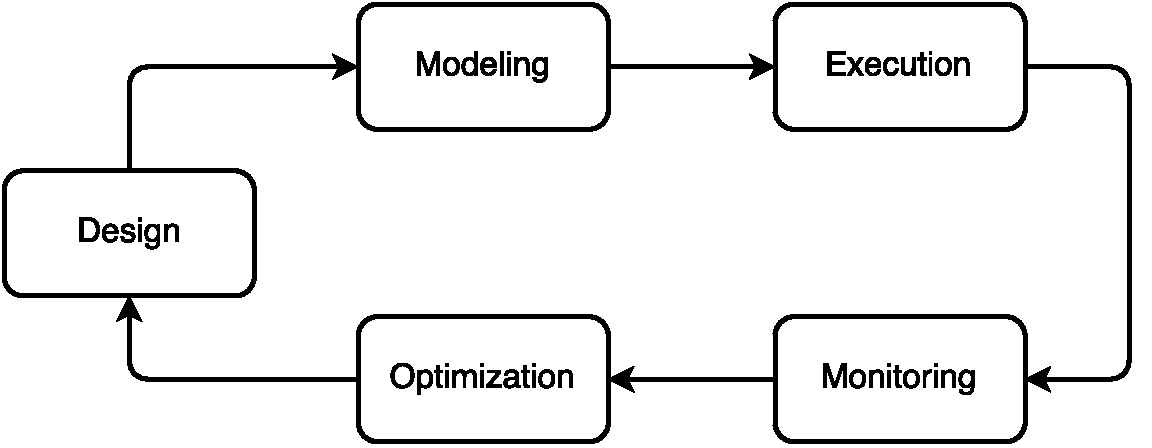
\includegraphics [width= \textwidth]{bpmlc.pdf}
	\caption{Business Process Life Cycle \cite{Wikipedia2016}}
	\label{fig:businessprocesslifecycle}
\end{figure}

\subsection{Organizational Intention Transparency (R1)}
An intention can be broken down into definitive actionable components or sub-intentions upon which individual resources can act. When these lower level sub-intentions are made achievable for individual resources, they can be combined to provide successful execution of higher level intention. Different organizational members can observe lower level and higher level intentions in their organizations based on the privileges provided to them. Intentions are traceable in the different levels of the organizational hierarchy. This means that the status of each intention can be accessed by members in different levels of the organizations based on their privilege. This level of transparency within an organization reduces inefficiencies in intention execution, and is a key factor in attracting and retaining high performers in the labor market \cite{McManus2007}. Requirement R1 has to be satisfied in the design phase itself as the designing of intentions, sub-intentions, strategies and privileges provided to participants are decided before the modeling phase. The main pre-requisites for this requirement are intentions can be refinable into sub-intentions and organizational members can view intentions at different levels based on their privilege. 

\subsection{Organizational Intention Resource-based Cost Estimation (R2)}
Linking intentions with strategies enable us a cost estimation for each intention. This is because intentions are realized through some strategies, then strategies are associated with organizational capabilities which in turn is associated with organizational resources. Cost is estimated in a recursive manner which has been explained in detail with an example in the following Chapter \ref{chap:approach}. To incorporate the cost estimation of intentions, we have to understand the recursive structure of the intentions associated with strategies. Since intentions are defined hierarchically, they can contain and extend intentions. Here strategy represents a means for achieving the intention. Further on, the cost of a strategy can be analyzed using the costs of derived sub-intentions, process definitions and so on. Including resources cost in intention cost calculation is important. This is achieved by associating resource models' cost with process models' cost. The recursion is stopped when the intention derivation process reaches the operational level. At the moment an intention is achieved, some resources should be allocated to maintain the desired state \cite{Mandic2010}. Allocation of resources is mainly done at the operational level,hence requirement R2 has to be satisfied during the modeling phase. Though, in design phase we can know the intentions and required resources but the developed editor can calculate the intention resource-based cost during modeling phase. The pre-requisites for this requirement to be satisfied are intention with recursive nature including its associated sub-intentions, strategies and resources.  

\subsection{Organizational Intention Achieve-ability Estimation (R3)}
The sub-intentions are projections of their super intentions, and satisfaction of the sub-intentions ensures satisfaction of the super intentions. Hence validity of an organizational intention is achievable when the intentions can be refined by defining sub-intentions, which can then be defined recursively as strategy and then to independent informal process models. Lower-level requirements can be validated against higher-level intentions, thus enabling validation of strategic alignment of  higher level intentions. The objectives of business strategy are found in the highest levels of the intention model \cite{Bleistein2006}.Requirement R3  can be found during the modeling phase of the process  as intention achieve-ability estimations are done before starting the execution of the intention based on the related intentions. For an intention to be achieve-able it should have a valid achieve-able recursive structure i.e., when a intention's sub-intentions are achieve-able then the main intention is also achieve-able. 

\subsection{Intention Oriented Working Style (R4)}
As each member of the organization is aware of the higher level and lower level intentions, he can engage for explicit intentions. Intention orientation is the degree to which a person or organization focuses on tasks and the end results of those tasks. Strong intention orientation advocates that focus on a task is more. Such a focused task ends in a result, favorable to both employees and organization. Those with strong intention orientation will be able to accurately judge the effects of reaching the intention as well as the ability to fulfill that particular intention with current resources and skills \cite{Lacom}. The distinction between explicit knowledge of each sub intentions should not be seen as a division but rather as a continuum which aligns towards achieving the higher level intention. Though requirement R4 is a part of requirement R1, R4 happens during modeling phase due to the dynamic nature of informal process. The pre-requisite for this requirement is system should allow to model intentions and its associated entities. 

\subsection{Participative Organizational Modeling (R5)}
 Different members of an organization participate to create organizational intentions, as a result intentions are shaped based on all members but directed by the executives. The  social  extension  of  a  business  process  can  be  regarded  as  a  process optimization phase, where the organization seeks efficiency  by  extending  the  reach  of  a  business  process  to  a  broader  class  of  stakeholders \cite{Brambilla2012}. Requirement R5 would be done at the execution phase as the input from different members of the organization are provided during the process execution. Since the list of participants who can have the privileges such as own/edit/follow/view access to the models can be determined beforehand this requirement is also satisfied during the design and modeling phases. The pre-requisite for this requirement is, the system should provide facility for different members of the organization to participate. 
 
 \subsection{Re-use of Organizational Knowledge (R6)}
 Intentions specific solutions can be extracted as abstract re-usable entities, organizational strategy patterns and can be re-used in multiple context definitions. These field tested solutions are made as descriptive model informations which can be re-used.  Re-using the informations as models from the previous executions trims out the model designing time \cite{Yu2000}. This requirement is satisfied during the design phase itself. This is because during the design phase itself business experts determine which models to re-use. The pre-requisite for this requirement is the system should provide facility to store the final state of models.

\begin{table} [htbp]
	\centering
	\begin{tabular} {p{2.5cm}p{3cm}p{8cm}}
		\toprule
		\textbf{Requirement} & \textbf{Requirement Satisfaction Phase} & \textbf{Pre-requisites}    \\
		\midrule                                                                                                               
		R1    & Design phase    &(1) Main intention can be refinable into sub-intentions, (2) Organizational members can view the intentions at different levels    \\ 
		
		R2   & Modeling phase    &(1) Intention cost estimation that includes all recursive sub-intentions, strategies and resources \\         
			
		R3   & Modeling phase       &(1) Each sub-intention should  be achievable and valid \\      
		
		R4   & Modeling and Execution phases     &(1) Satisfaction of R1, (2) Understanding of the intentions and how they can be reached \\                         
			
		R5  &Design, Modeling and Execution phases  &(1) Satisfaction of R1, (2) Intention is modeled based on the inputs provided by different members of the organization               \\ 
		
		R6   & Design phase         &(1) Organization knowledge should be stored as models \\        
		
		\bottomrule
	\end{tabular}
	\caption{Requirements Analysis}
	\label{tab:subrequirements}
\end{table}

%%%%%%%%%%%%%%%%%%%%%%%%%%%%%%%%%%%%%%%%%%%%%%%%%%%%%%%%%%%%%%%%%%%%%%%%%
\section{Literature Review}
\label{sec:literaturereview}
%%%%%%%%%%%%%%%%%%%%%%%%%%%%%%%%%%%%%%%%%%%%%%%%%%%%%%%%%%%%%%%%%%%%%%%%%
In the literature, several work has been done in order to support and automate the business process modeling such as strategy-driven \cite{bider2005strategy}, activity-centric\cite{Yarosh2009}, activity-oriented \cite{Reijers2006}, artifact-centric \cite{Cohn2009}, capability-driven \cite{Stirna2012}, archimate \cite{Aldea2015} and subject-oriented \cite{Fleischmann2013}.  A detailed description about these approaches and their degree of satisfying the requirements mentioned in Section \ref{sec:requirementssupoorting} has also been provided. 

\subsection{Strategy-Driven} 
This approach \cite{bider2005strategy} defines business process in terms of goals and strategies in order to achieve the goals. It also uses map representation system that contains goals and strategies. In this approach the details regarding visibility of goals has not been addressed, hence requirement R1 is not satisfied. Also details about cost of achieving a goal through a strategy has also been not addressed, hence requirement R2 is also not satisfied. The requirement R3 contradicts with the process rule of this approach which states that "There is no goal/strategy in the map that can be considered as the subset of another one". Requirement R4 is also not satisified due to the fact that this approach follows strategy driven modeling. Information about participation of different members has also not been metioned, hence requirement R5 is also not met. This approach addresses the requirement R6, as it supports re-usability of the map components in different maps. 

\subsection{Activity-Centric} 
The activity-centric approach \cite{Yarosh2009} also supports knowledge workers by providing shared activity constructs as a computational unit for organizing the work. This approach provides team level view of past and ongoing work and also supports propogation of completed activities to the existing activities. Hence requirement R1 is partially met. The information about cost of achieving a goal or activity has not been mentioned. Thus requirement R2 is not satisfied. In this approach, activities support objectives at various levels of granularity and thus requirement R4 is met. Since the main focus of this approach is activity, it has not provided any information regarding working style based on goals, instead the working style is based on activities. Hence requirement R5 is not met. Cross activity overview pattern is one of the pattern described in this approach which does unifying work across the team members, hence requirement R5 is addressed. Since this approach also supports reusable activity patterns requirement R6 is also met. 
 
\subsection{Activity-Oriented} 
The activity-oriented approach \cite{Reijers2006} is traditional workflow management approach where the main focus unit is business process' activity rather than strategy. In traditional workflows the concept of "process view" from different levels of an organisation not addressed, thus requirement R1 is not addressed. The details about cost calculation is not mentioned, hence requirement R2 is also not satisfied. Though this approach does not support sub-processes directly, it provides support for plugging in sub process extensions, this satisfies requirement R3. From goal oriented to activity oriented working style, so the working style is based on activities and not on goals. Thus requirement R4 is not addressed. Traditional workflow models like BPMN do not support participative modeling, but extensions like social-BPM supports social interactions. Hence requirement R5 is addressed. Re-using of existing activities is not addressed, thus requirement R6 is not addressed.  

\subsection{Artifact-Centric} 
The artifact-centric approach \cite{Cohn2009} combines business data as artifacts and business process in a holistic way. This approach clearly states that artifacts "views" is not addressed, thus requirement R1 is not satisfied. The requirement R2 which is about cost calculation is not addressed. This approach allows modularity and componentization of business operations at various levels, hence requirement R3 is satisfied. Requirement R4  is partially met as the process evolves through a series of intermediate goals. Requirement R5 is not met due to the fact that concept of social organizational modeling is not addressed. Requirement R6 is partially met because, only the concepts of modularization, componentization at various levels of abstraction has been discussed but reuse of components has not been addressed.

\subsection{Capability-Driven} 
The capability driven approach \cite{Stirna2012} also proposes to support the changing environment of organizations. But in this approach there is no information about the visibility of goals has been addressed. Hence requirement R1 is not met. This approach claims that, it overcomes the challenge of high cost in developing applications but there is no clear details about how cost calculation is done, hence requirement R2 is not addressed. In this approach, the top goal is refined into a number of sub-goals, then each sub-goal is lined to one or several KPIs. Thus requirement R3 is met. Since visibility of goals is not addressed, the details about explicit goals which is requirement R4 is not addressed. Requirement R5 is not addressed as the concept of multiple resources working together is not described. Reuse and execution of capability delivery pattern has been addressed, this meets requirement R6. 

\subsection{ArchiMate} 
This approach \cite{Aldea2015}, investigates if ArchiMate modeling language tool can be used to model strategies and also addresses the properties of Archimate. This apporach provides visibility of whole process, supports "viewpoints" in different levels of modeling. Thus requirement R1 is addressed. Requirement R2 which is cost of achieving each goal is not addressed. The approach provides three levels of modeling i.e., business, application, and technology, thus requirement R3 is partially met. This approach provides visibility of whole process which supports explicit goals but ArchiMate modeling language is not very easy to use to model multiple strategies with goal concept, thus requirement R4 is partially met. Requirement R5 is addressed as it supports different resources participation at different levels. Requirement R6 is also addressed as re-use of existing models is supported. 

\subsection{Subject-Oriented} 
This approach \cite{Fleischmann2013} supports multi-agent business process models that improves efficiency of the business logics. In this approach, requirement R1 is partially addressed  as S-BPM shows process view of who communicates with whom but not how the process advances or if it terminates at all. Requirement R2 which is cost of achieving each goal is not addressed. Requirement R3 is addressed as the main process net can be divided into sub-nets. Requirement R4 is not addressed, as the concept of explicit goals is not described. S-BPM emphasises "subjects" in a process as a decenrtalised, interacting entities thus requirement R5 is addressed. Requirement R6 which is about re-using of existing knowledge is not addressed. 

\subsection {Evaluation of the Approach}
 The approach \textit{Adaptive Case Management}, proposed by Hermann et. al \cite{Herrmann2011} bridges the gap between business processes management and flexibility in adapting knowledge intensive processes by defining activities and re-using created activity structure. When the required activities changes dynamically, capturing them for re-use are not helpful \cite{Sungur2015}. Though the approach \textit{Ad-hoc and Collaborative Processes} proposed by Dustdar et. al. overcomes the challenges in process aware collaborations, defining activities in a ad-hoc fashion does not support human actor in various cases \cite{Sungur2015}. Also the approach proposed in Chapter \ref{chap:approach} serves as a complementary to the above discussed  approaches.  This is because every existing approach satisfies one or few of the requirements even though not all requirements are satisfied. The Table \ref{tab:evaluationoftheapproach}, shows the extent of requirements satisfied by the selected existing approaches. 

\begin{center}
	\begin{longtable}{p{6cm}p{1.5cm}p{1.5cm}p{1.5cm}p{1.5cm}p{1.5cm}p{1.5cm}} 
		\toprule 
		\textbf{Approach} & \textbf{R1}  & \textbf{R2}  & \textbf{R3}  & \textbf{R4}  & \textbf{R5} & \textbf{R6} \\
		\midrule
		\endfirsthead
		
		Strategy-Driven & No  & No  & No  & Partial  & No  & Yes\\
		Activity-Centric   & Partial   & No  & Yes  & Partial  & No  & Yes \\
		Activity-Oriented    & No  & No  & Yes  & No   & Yes  & No \\
		Artifact-Centric    & No  & No  & Yes  & No & Partial  & Partial \\ 
		Capability-Driven   & No  & No  & Yes  & No  & No  & Yes\\
		ArchiMate  & Yes  & No  & Partial  & Partial  & Yes  & Yes \\
		Subject-Oriented   &Partial  & No  & Yes  & No   & Yes   & No\\
		
		\bottomrule
		\caption{Evaluation of the Approach}
		\label{tab:evaluationoftheapproach}
	\end{longtable}	
\end{center}
Legend :
\begin{description}
	\item[Yes]      Requirement is addressed in the selected approach
	\item[No]       Requirement is not addressed in the selected approach
	\item[Partial]  Requirement is partially addressed in the selected approach
\end{description}



 


